% include the figures path relative to the master file
\graphicspath{{./content/intro/figures/}}
\section{Setting the polarimetric camera for robotics}
\label{sec:rosify}

As mentioned previously, in this work we use a \gls{dofp} polarimetric camera,
to be exact \textit{IMPREX Bobcat GEV polarimetric camera}.
This camera has the advantage to capture four different linearly polarized
measure in one image, due to their micropolarizer and pixelated polarized
filter array (see Fig.~\ref{fig:dofp-sensor}).
Therefore each capture image leads to four linearly polarized sub-image $I_0$,
$I_{45}$, $I_{135}$, $I_{90}$.
Using these four measurements, the polarized state of the incident light is
calculated in terms of stokes parameters~\cite{goldstein2017polarized}, which
are used thereafter to calculate polarized parameters such as \gls{aop} and
\gls{dopl} (see Eq.~\ref{eq:stokes}).

\begin{figure}
  \centering
  \includegraphics[width=0.3\textwidth]{./content/intro/figures/dofp-sensor-0-45-135-90.jpg}
  \caption{Structure of \gls{dofp} sensors. Using this sensor four linearly
    polarized image corresponding to the four orientation of the polarized
    filters is acquired instantly}
    \label{fig:dofp-sensor}
\end{figure}

\begin{figure*}
  \centering
  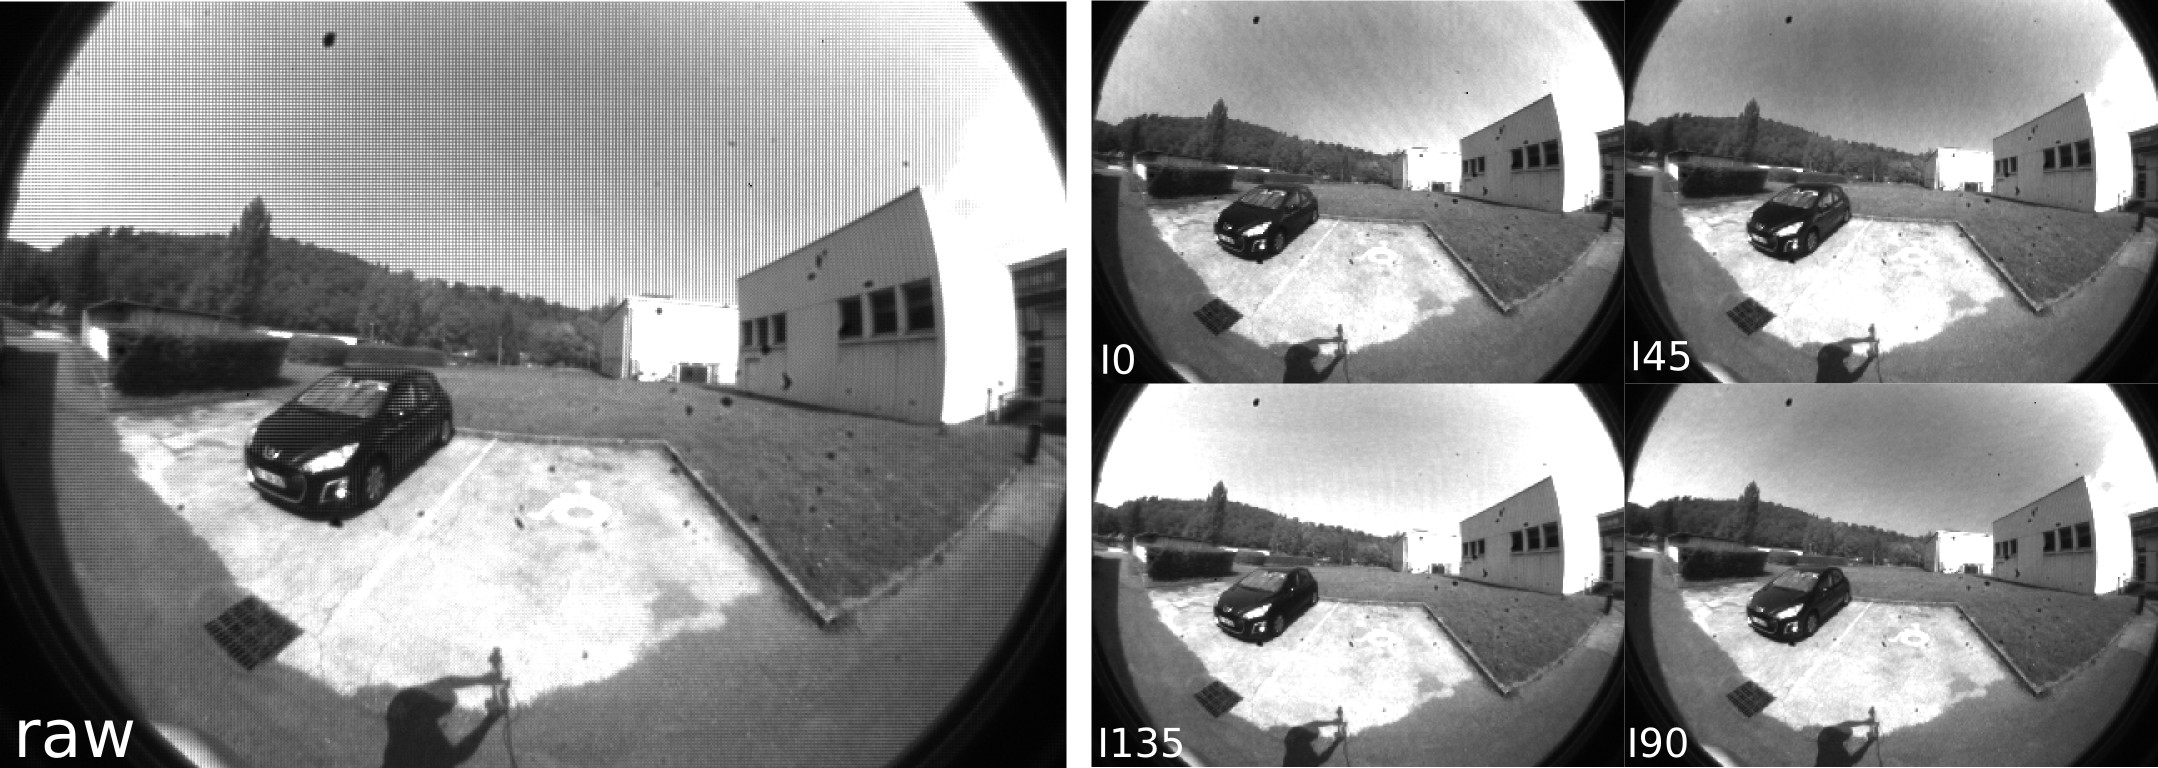
\includegraphics[width=0.7\textwidth]{./content/intro/figures/raw-sp.jpg}
  \caption{A raw image captured with fisheye lens, and the extracted four
    linearly polarized images ($I_0, I_{45}, I_{135}, I_{90}$)}
  \label{fig:raw-sp}
\end{figure*}

\begin{figure*}
  \centering
  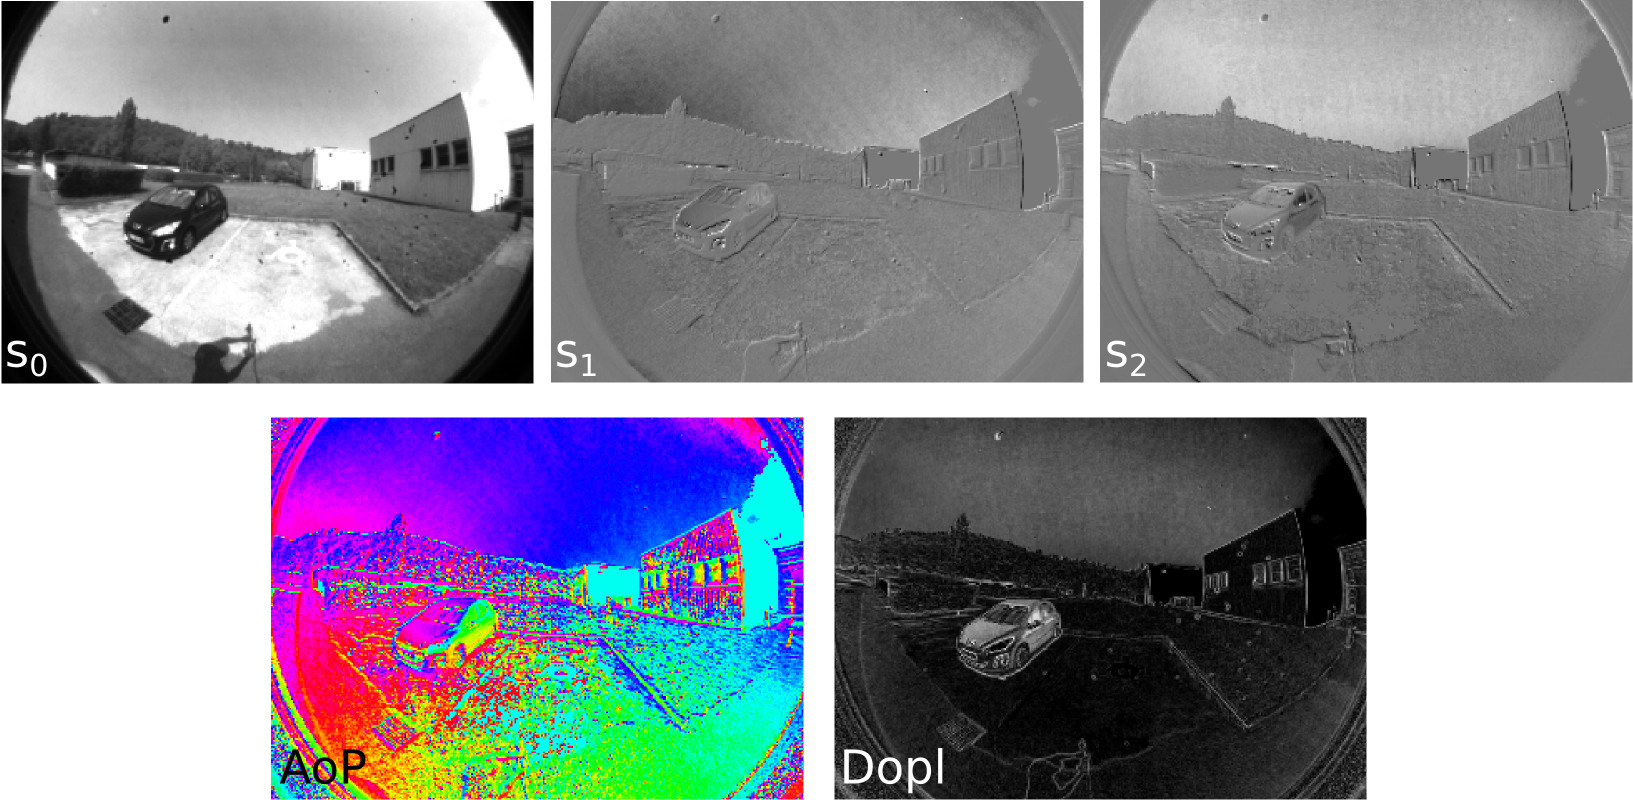
\includegraphics[width=0.7\textwidth]{./content/intro/figures/stokes_aop_dop.jpg}
  \caption{Calculated stokes parameters ($s_0, s_1, s_2$), \gls{aop}, and
    \gls{dopl} images. For visualization purpose, \gls{aop} is represented in
    $hsv$ color space.}
  \label{fig:stokes-aop-dop}
\end{figure*}




\begin{subequations}
  \begin{align}
    \label{eq:stokes1}
    \small
    s_0 & = (I_0 + I_{45} + I_{135} + I_{90})/4\\ \nonumber
    s_1 & = I_0 - I_{90} \\ \nonumber
    s_2 & = I_{45} - I_{135} \nonumber
  \end{align}
  \begin{align}
    \label{eq:stokes2}
    \small
    \gls{aop} & = \alpha = 0.5 \arctan(s_2/s_1) \\ \nonumber
    \gls{dopl} & = \rho_l = \frac{\sqrt{s_2^{2} + s_1^{2}}}{s_0} \nonumber
  \end{align}
  \label{eq:stokes}
\end{subequations}

From the raw images ($640\times460$) captured by the camera, the sub-images can
be extracted directly using super-pixel method that leads to four images, half
of the size of the raw image, or can be interpolated to the full
size~\cite{ratliff2009interpolationmicrogrid,gao2011bilinearpolarimeters}.  The
super-pixel method was used for the results presented in this paper. Being
interested in large-field of view, a fisheye lens of 180-degree was used on the
camera, \textcolor{red}{information of the lens}.

An example of captured raw image, the linearly polarized
images and subsequently the three stokes parameters and polarized information
is shown in Fig.~\ref{fig:raw-sp}~$\&$~\ref{fig:stokes-aop-dop}.

The \textit{IMPREX Bobcat GEV} camera operates using eBus SDK-pleora driver and
libraries~\cite{eBus}. To be able to use the camera integrated with other
sensors, in the robotic field, we have created a ROS
package, pleora-polarcam~\cite{pleora_polarcam}.
Initiating from Iralab photonfocus driver~\cite{ira}, pleora-polarcam package
is adapted for Imperex polarimetric cameras.
Using this package the user can easily \text{roslaunch} or \text{rosrun} the
camera and beside, buffering and saving the raw data, process the stokes and
polarized parameters.



%%%Local Variables:
%%% mode: latex
%%% TeX-master: t
%%% End:
